\documentclass[9pt,ignorenonframetext,]{beamer}
\setbeamertemplate{caption}[numbered]
\setbeamertemplate{caption label separator}{: }
\setbeamercolor{caption name}{fg=normal text.fg}
\beamertemplatenavigationsymbolsempty
\usepackage{lmodern}
\usepackage{amssymb,amsmath}
\usepackage{ifxetex,ifluatex}
\usepackage{fixltx2e} % provides \textsubscript
\ifnum 0\ifxetex 1\fi\ifluatex 1\fi=0 % if pdftex
\usepackage[T1]{fontenc}
\usepackage[utf8]{inputenc}
\else % if luatex or xelatex
\ifxetex
\usepackage{mathspec}
\else
\usepackage{fontspec}
\fi
\defaultfontfeatures{Ligatures=TeX,Scale=MatchLowercase}
\fi
% use upquote if available, for straight quotes in verbatim environments
\IfFileExists{upquote.sty}{\usepackage{upquote}}{}
% use microtype if available
\IfFileExists{microtype.sty}{%
\usepackage{microtype}
\UseMicrotypeSet[protrusion]{basicmath} % disable protrusion for tt fonts
}{}
\newif\ifbibliography
\usepackage{color}
\usepackage{fancyvrb}
\newcommand{\VerbBar}{|}
\newcommand{\VERB}{\Verb[commandchars=\\\{\}]}
\DefineVerbatimEnvironment{Highlighting}{Verbatim}{commandchars=\\\{\}}
% Add ',fontsize=\small' for more characters per line
\usepackage{framed}
\definecolor{shadecolor}{RGB}{248,248,248}
\newenvironment{Shaded}{\begin{snugshade}}{\end{snugshade}}
\newcommand{\KeywordTok}[1]{\textcolor[rgb]{0.13,0.29,0.53}{\textbf{{#1}}}}
\newcommand{\DataTypeTok}[1]{\textcolor[rgb]{0.13,0.29,0.53}{{#1}}}
\newcommand{\DecValTok}[1]{\textcolor[rgb]{0.00,0.00,0.81}{{#1}}}
\newcommand{\BaseNTok}[1]{\textcolor[rgb]{0.00,0.00,0.81}{{#1}}}
\newcommand{\FloatTok}[1]{\textcolor[rgb]{0.00,0.00,0.81}{{#1}}}
\newcommand{\ConstantTok}[1]{\textcolor[rgb]{0.00,0.00,0.00}{{#1}}}
\newcommand{\CharTok}[1]{\textcolor[rgb]{0.31,0.60,0.02}{{#1}}}
\newcommand{\SpecialCharTok}[1]{\textcolor[rgb]{0.00,0.00,0.00}{{#1}}}
\newcommand{\StringTok}[1]{\textcolor[rgb]{0.31,0.60,0.02}{{#1}}}
\newcommand{\VerbatimStringTok}[1]{\textcolor[rgb]{0.31,0.60,0.02}{{#1}}}
\newcommand{\SpecialStringTok}[1]{\textcolor[rgb]{0.31,0.60,0.02}{{#1}}}
\newcommand{\ImportTok}[1]{{#1}}
\newcommand{\CommentTok}[1]{\textcolor[rgb]{0.56,0.35,0.01}{\textit{{#1}}}}
\newcommand{\DocumentationTok}[1]{\textcolor[rgb]{0.56,0.35,0.01}{\textbf{\textit{{#1}}}}}
\newcommand{\AnnotationTok}[1]{\textcolor[rgb]{0.56,0.35,0.01}{\textbf{\textit{{#1}}}}}
\newcommand{\CommentVarTok}[1]{\textcolor[rgb]{0.56,0.35,0.01}{\textbf{\textit{{#1}}}}}
\newcommand{\OtherTok}[1]{\textcolor[rgb]{0.56,0.35,0.01}{{#1}}}
\newcommand{\FunctionTok}[1]{\textcolor[rgb]{0.00,0.00,0.00}{{#1}}}
\newcommand{\VariableTok}[1]{\textcolor[rgb]{0.00,0.00,0.00}{{#1}}}
\newcommand{\ControlFlowTok}[1]{\textcolor[rgb]{0.13,0.29,0.53}{\textbf{{#1}}}}
\newcommand{\OperatorTok}[1]{\textcolor[rgb]{0.81,0.36,0.00}{\textbf{{#1}}}}
\newcommand{\BuiltInTok}[1]{{#1}}
\newcommand{\ExtensionTok}[1]{{#1}}
\newcommand{\PreprocessorTok}[1]{\textcolor[rgb]{0.56,0.35,0.01}{\textit{{#1}}}}
\newcommand{\AttributeTok}[1]{\textcolor[rgb]{0.77,0.63,0.00}{{#1}}}
\newcommand{\RegionMarkerTok}[1]{{#1}}
\newcommand{\InformationTok}[1]{\textcolor[rgb]{0.56,0.35,0.01}{\textbf{\textit{{#1}}}}}
\newcommand{\WarningTok}[1]{\textcolor[rgb]{0.56,0.35,0.01}{\textbf{\textit{{#1}}}}}
\newcommand{\AlertTok}[1]{\textcolor[rgb]{0.94,0.16,0.16}{{#1}}}
\newcommand{\ErrorTok}[1]{\textcolor[rgb]{0.64,0.00,0.00}{\textbf{{#1}}}}
\newcommand{\NormalTok}[1]{{#1}}
\usepackage{graphicx,grffile}
\makeatletter
\def\maxwidth{\ifdim\Gin@nat@width>\linewidth\linewidth\else\Gin@nat@width\fi}
\def\maxheight{\ifdim\Gin@nat@height>\textheight0.8\textheight\else\Gin@nat@height\fi}
\makeatother
% Scale images if necessary, so that they will not overflow the page
% margins by default, and it is still possible to overwrite the defaults
% using explicit options in \includegraphics[width, height, ...]{}
\setkeys{Gin}{width=\maxwidth,height=\maxheight,keepaspectratio}

% Prevent slide breaks in the middle of a paragraph:
\widowpenalties 1 10000
\raggedbottom

\AtBeginPart{
\let\insertpartnumber\relax
\let\partname\relax
\frame{\partpage}
}
\AtBeginSection{
\ifbibliography
\else
\let\insertsectionnumber\relax
\let\sectionname\relax
\frame{\sectionpage}
\fi
}
\AtBeginSubsection{
\let\insertsubsectionnumber\relax
\let\subsectionname\relax
\frame{\subsectionpage}
}

\setlength{\parindent}{0pt}
\setlength{\parskip}{6pt plus 2pt minus 1pt}
\setlength{\emergencystretch}{3em}  % prevent overfull lines
\providecommand{\tightlist}{%
\setlength{\itemsep}{0pt}\setlength{\parskip}{0pt}}
\setcounter{secnumdepth}{0}

\title{STA305/1004 - Review of Statistical Theory}
\date{January 11, 2017}

\begin{document}
\frame{\titlepage}

\begin{frame}[fragile]{Data}

Experimental data describes the outcome of the experimental run. For
example 10 successive runs in a chemical experiment produce the
following data:

\begin{Shaded}
\begin{Highlighting}[]
\KeywordTok{set.seed}\NormalTok{(}\DecValTok{100}\NormalTok{)}
\CommentTok{# Generate a random sample of 5 observations }
\CommentTok{# from a N(60,10^2)}
\NormalTok{dat <-}\StringTok{ }\KeywordTok{round}\NormalTok{(}\KeywordTok{rnorm}\NormalTok{(}\DecValTok{5}\NormalTok{,}\DataTypeTok{mean =} \DecValTok{60}\NormalTok{,}\DataTypeTok{sd =} \DecValTok{10}\NormalTok{),}\DecValTok{1}\NormalTok{) }
\NormalTok{dat}
\end{Highlighting}
\end{Shaded}

\begin{verbatim}
## [1] 55.0 61.3 59.2 68.9 61.2
\end{verbatim}

\end{frame}

\begin{frame}[fragile]{Distributions}

Distributions can be displayed graphically or numerically.

A histogram is a graphical summary of a data set.

\begin{Shaded}
\begin{Highlighting}[]
\KeywordTok{summary}\NormalTok{(dat)}
\end{Highlighting}
\end{Shaded}

\begin{verbatim}
##    Min. 1st Qu.  Median    Mean 3rd Qu.    Max. 
##   55.00   59.20   61.20   61.12   61.30   68.90
\end{verbatim}

\end{frame}

\begin{frame}[fragile]{Distributions}

\begin{Shaded}
\begin{Highlighting}[]
\KeywordTok{hist}\NormalTok{(dat)}
\end{Highlighting}
\end{Shaded}

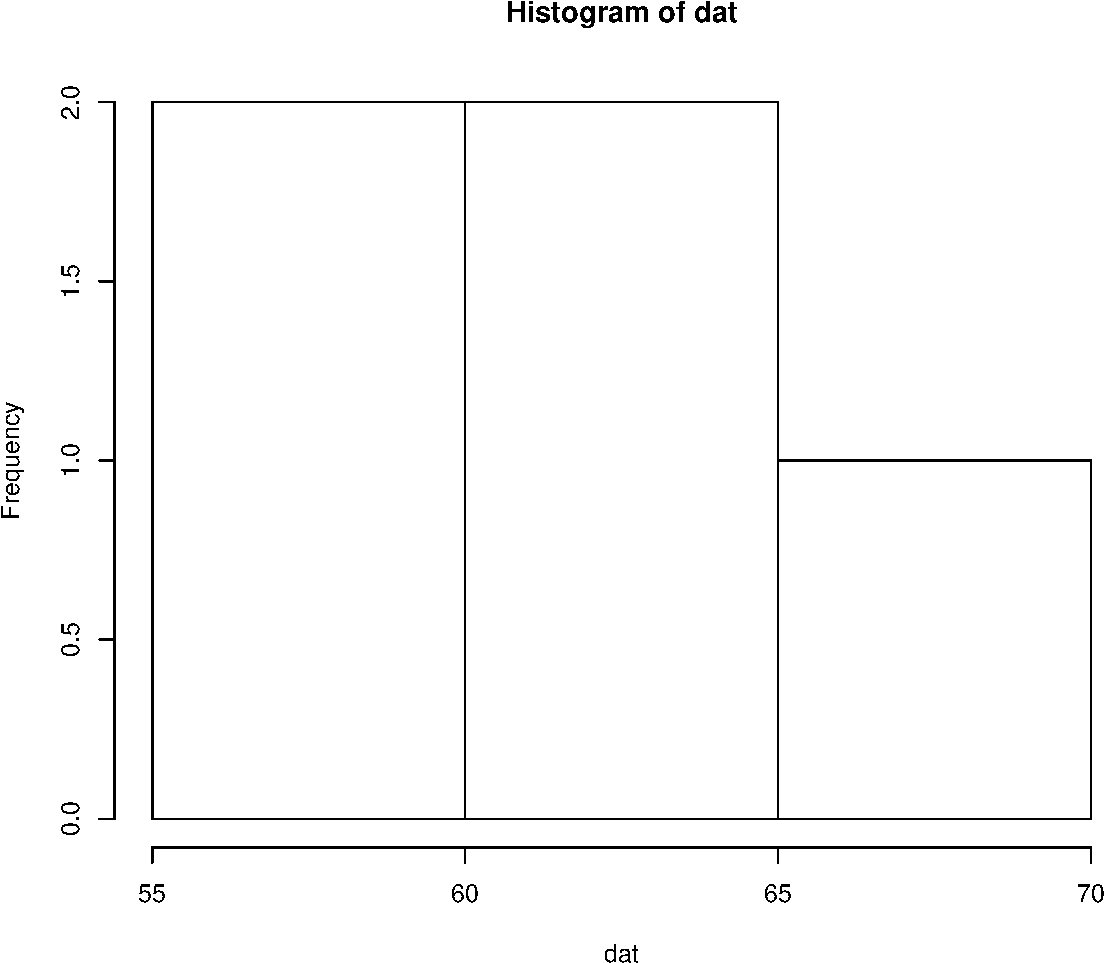
\includegraphics{class2-jan11_files/figure-beamer/unnamed-chunk-3-1.pdf}

\end{frame}

\begin{frame}{Distributions}

\begin{itemize}
\tightlist
\item
  The total aggregate of observations that might occur as a result of
  repeatedly performing a particular operation is called a
  \textbf{population} of observations.
\item
  The observations that actually occur are a \textbf{sample} from the
  population.
\end{itemize}

\end{frame}

\begin{frame}{Continuous Distributions}

\begin{itemize}
\item
  A continuous random variable \(X\) is fully characterized by it's
  density function \(f(x)\).
\item
  \(f(x) \ge 0\), \(\thinspace f\) is piecewise continuous, and
  \(\int_{-\infty}^{\infty}f(x)dx=1\).
\item
  The cumulative distribution function (CDF) of \(X\) is defined as:
\end{itemize}

\[ F(x)=P(X \le x)=\int_{-\infty}^{x}f(x)dx.\]

\end{frame}

\begin{frame}[fragile]{Continuous Distributions}

\begin{itemize}
\tightlist
\item
  If \(f\) is continuous at \(x\) then \(F'(x)=f(x)\) (fundamental
  theorem of calculus).\\
\item
  The CDF can be used to calculate the probability that \(X\) falls in
  the interval \((a,b)\). This is the area under the density curve which
  can also be expressed in terms of the CDF:
\end{itemize}

\[P\left(a < X < b\right)=\int_{a}^{b}f(x)dx=F(b)-F(a).\]

\begin{itemize}
\tightlist
\item
  In R a list of all the common distributions can be obtained by the
  command \texttt{help("distributions")}.
\item
  For example, the normal density and CDF are given by \texttt{dnorm()}
  and \texttt{pnorm()}.
\end{itemize}

\end{frame}

\begin{frame}[fragile]{Continuous Distributions}

100 observations (using \texttt{rchisq()}) from a Chi-square
distribution on 10 degrees of freedom \(\chi^2_{10}\). The density
function of the \(\chi^2_{10}\) is superimposed over the histogram of
the sample.

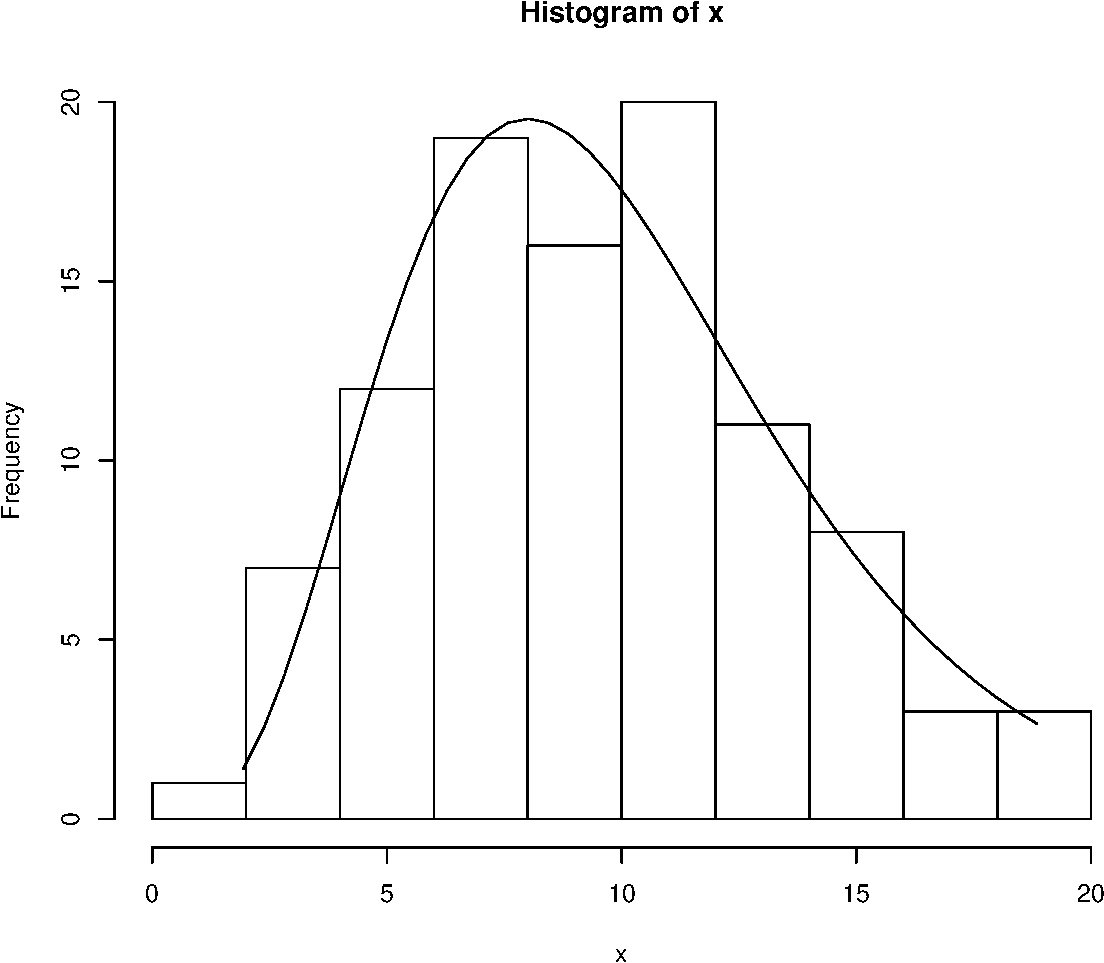
\includegraphics{class2-jan11_files/figure-beamer/unnamed-chunk-4-1.pdf}

\end{frame}

\begin{frame}{Randomness}

\begin{itemize}
\tightlist
\item
  A random drawing is where each member of the population has an equal
  chance of being selected.
\item
  The hypothesis of random sampling may not apply to real data.
\item
  For example, cold days are usually followed by cold days.\\
\item
  So daily temperature not directly representable by random drawings.
\item
  In many cases we can't rely on the random sampling property although
  design can make this assumption relevant.
\end{itemize}

\end{frame}

\begin{frame}{Parameters and Statistics}

What is the difference between a parameter and a statistic?

\begin{itemize}
\tightlist
\item
  A parameter is a population quantity and a statistic is a quantity
  based on a sample drawn from the population.
\end{itemize}

Example: The population of all adult (18+ years old) males in Toronto,
Canada.

\begin{itemize}
\tightlist
\item
  Suppose that there are \(N\) adult males and the quantity of interest,
  \(y\), is age.\\
\item
  A sample of size \(n\) is drawn from this population.\\
\item
  The population mean is \(\mu=\sum_{i=1}^N y_i /N\).
\item
  The sample mean is \({\bar y}=\sum_{i=1}^n y_i /n\).
\end{itemize}

\end{frame}

\begin{frame}{Residuals and Degress of Freedom}

\(y_i-{\bar y}\) is called a residual.

\begin{itemize}
\tightlist
\item
  Since \(\sum (y_i-{\bar y})=0\) any \(n-1\) completely determine the
  the last observation.\\
\item
  This is a constraint on the the residuals.\\
\item
  So \(n\) residuals have \(n-1\) degrees of freedom since the last
  residual cannot be freely chosen.
\end{itemize}

\end{frame}

\begin{frame}{The Normal Distribution}

The density function of the normal distribution with mean \(\mu\) and
standard deviation \(\sigma\) is:

\[ \phi(x)=\frac{1}{\sigma \sqrt{2\pi}}exp\left( \frac{-1}{2} \left(\frac{x-\mu}{\sigma}\right)^2\right)\]

The cumulative distribution function (CDF) of a \(N(0,1)\) distribution,

\[ \Phi(x)= P(X<x)= \int_{-\infty}^x \phi(x)dx\]

\end{frame}

\begin{frame}[fragile]{The Normal Distribution}

\begin{Shaded}
\begin{Highlighting}[]
\NormalTok{x <-}\StringTok{ }\KeywordTok{seq}\NormalTok{(-}\DecValTok{4}\NormalTok{,}\DecValTok{4}\NormalTok{,}\DataTypeTok{by=}\FloatTok{0.1}\NormalTok{)}
\KeywordTok{plot}\NormalTok{(x,}\KeywordTok{dnorm}\NormalTok{(x),}\DataTypeTok{type=}\StringTok{"l"}\NormalTok{,}\DataTypeTok{main =} \StringTok{"The Standard Normal Distribution"}\NormalTok{, }
     \DataTypeTok{ylab=}\KeywordTok{expression}\NormalTok{(}\KeywordTok{paste}\NormalTok{(}\KeywordTok{phi}\NormalTok{(x))))}
\end{Highlighting}
\end{Shaded}

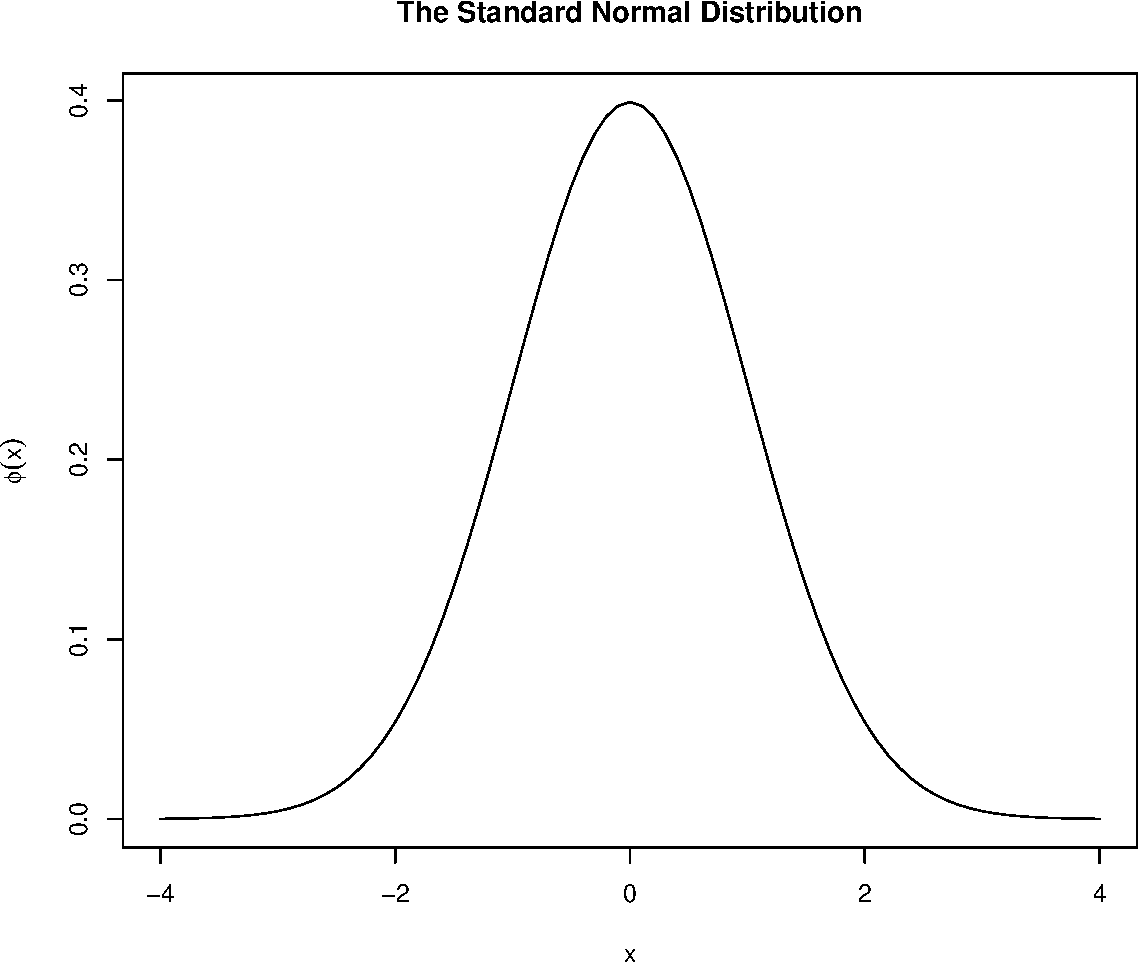
\includegraphics{class2-jan11_files/figure-beamer/unnamed-chunk-5-1.pdf}

\end{frame}

\begin{frame}[fragile]{The Normal Distribution}

\begin{Shaded}
\begin{Highlighting}[]
\KeywordTok{plot}\NormalTok{(x <-}\StringTok{ }\KeywordTok{seq}\NormalTok{(-}\DecValTok{2}\NormalTok{,}\DecValTok{2}\NormalTok{,}\DataTypeTok{by=}\FloatTok{0.1}\NormalTok{),}\KeywordTok{pnorm}\NormalTok{(x),}\DataTypeTok{type=}\StringTok{"l"}\NormalTok{,}
     \DataTypeTok{xlab=}\StringTok{"x"}\NormalTok{,}\DataTypeTok{ylab=}\KeywordTok{expression}\NormalTok{(}\KeywordTok{paste}\NormalTok{(}\KeywordTok{Phi}\NormalTok{(x))),}
     \DataTypeTok{main =} \StringTok{"Standard Normal Cumulative Distribution Function"}\NormalTok{)}
\end{Highlighting}
\end{Shaded}

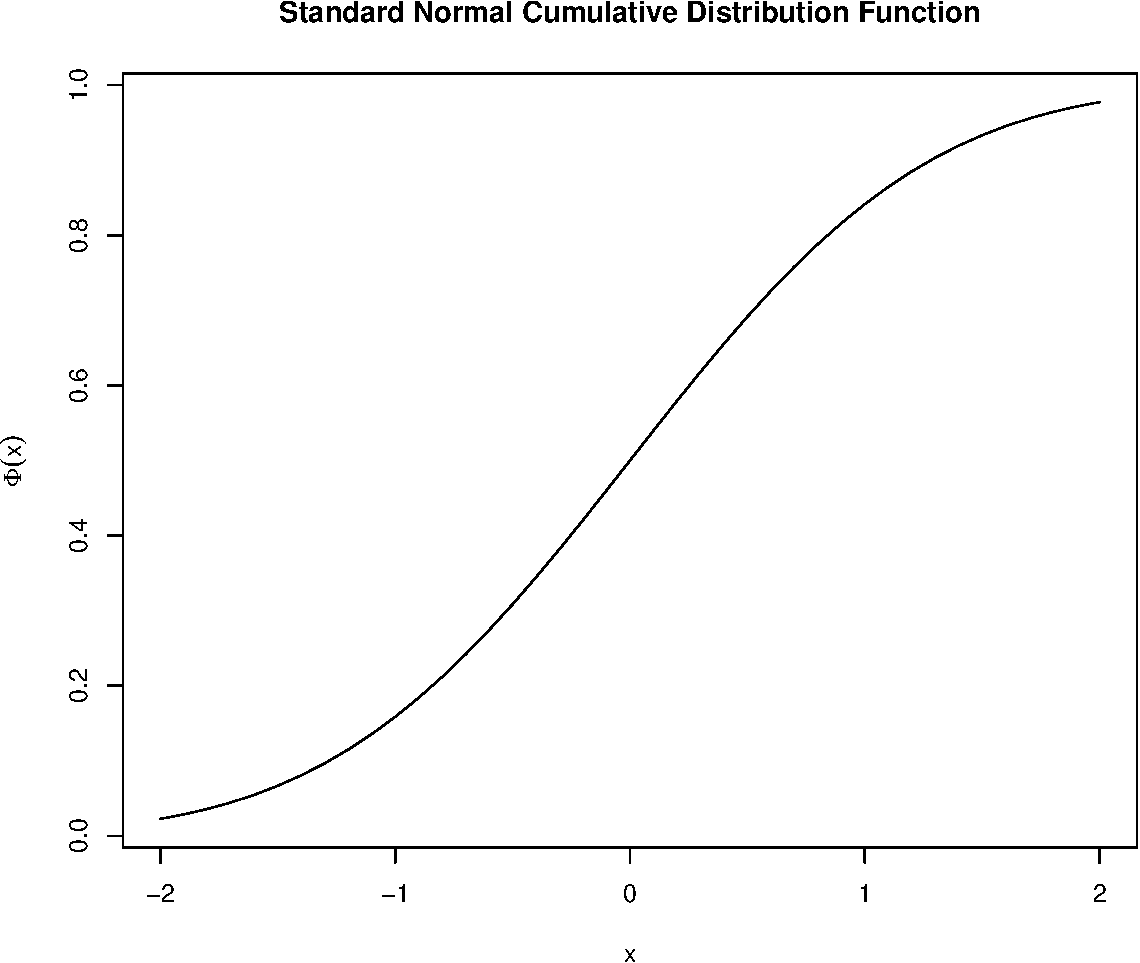
\includegraphics{class2-jan11_files/figure-beamer/unnamed-chunk-6-1.pdf}

\end{frame}

\begin{frame}{The Normal Distribution}

A random variable \(X\) that follows a normal distribution with mean
\(\mu\) and variance \(\sigma^2\) will be denoted by
\[X \sim N\left(\mu, \sigma^2\right).\]

If \(Y \sim N\left(\mu, \sigma^2\right)\) then \[Z \sim N(0,1),\] where
\[Z=\frac{Y-\mu}{\sigma}.\]

\end{frame}

\begin{frame}[fragile]{The Normal Distribution}

\(X \sim N(5,3)\). Use R to find \(P(4<X<6)\).

\begin{Shaded}
\begin{Highlighting}[]
\KeywordTok{pnorm}\NormalTok{(}\DecValTok{6}\NormalTok{,}\DataTypeTok{mean =} \DecValTok{5}\NormalTok{,}\DataTypeTok{sd =} \KeywordTok{sqrt}\NormalTok{(}\DecValTok{3}\NormalTok{))-}\KeywordTok{pnorm}\NormalTok{(}\DecValTok{4}\NormalTok{,}\DataTypeTok{mean =} \DecValTok{5}\NormalTok{,}\DataTypeTok{sd =} \KeywordTok{sqrt}\NormalTok{(}\DecValTok{3}\NormalTok{))}
\end{Highlighting}
\end{Shaded}

\begin{verbatim}
## [1] 0.4362971
\end{verbatim}

\end{frame}

\begin{frame}[fragile]{Normal Quantile Plots}

The following data are the weights from 11 tomato plants.

\begin{verbatim}
##  [1] 29.9 11.4 26.6 23.7 25.3 28.5 14.2 17.9 16.5 21.1 24.3
\end{verbatim}

Do the weights follow a Normal distribution?

\end{frame}

\begin{frame}[fragile]{Normal Quantile Plots}

A normal quantile plot in R can be obtained using \texttt{qqnorm()} for
the normal probability plot and \texttt{qqline()} to add the straight
line.

\begin{Shaded}
\begin{Highlighting}[]
\KeywordTok{qqnorm}\NormalTok{(tomato.data$pounds); }\KeywordTok{qqline}\NormalTok{(tomato.data$pounds)}
\end{Highlighting}
\end{Shaded}

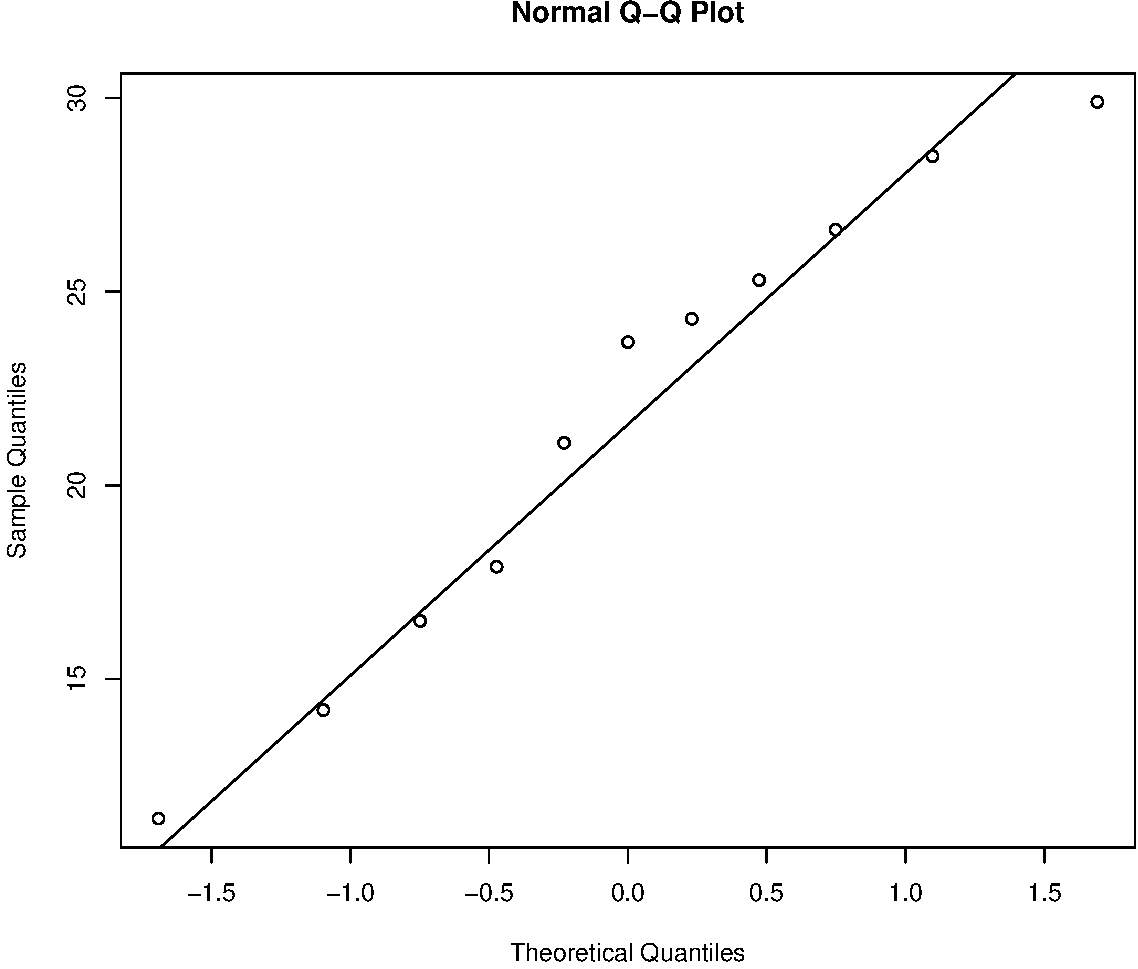
\includegraphics{class2-jan11_files/figure-beamer/unnamed-chunk-9-1.pdf}

\end{frame}

\begin{frame}{Central Limit Theorem}

The central limit theorem states that if \(X_1, X_2, ...\) is an
independent sequence of identically distributed random variables with
mean \(\mu=E(X_i)\) and variance \(\sigma^2=Var(X_i)\) then

\[ \lim_{n\to\infty} P\left(\frac{\bar X - \mu}{\frac {\sigma}{\sqrt n}} \leq x \right) = \Phi(x),\]

where \({\bar X} = \sum_{i=1}^{n} X_i/n\) and \(\Phi(x)\) is the
standard normal CDF. This means that the distribution of \({\bar X}\) is
approximately \(N\left(\mu,{\frac {\sigma}{\sqrt n}}\right)\).

\end{frame}

\begin{frame}{Central Limit Theorem}

Example: A fair coin is flipped 50 times. What is the distribution of
the average number of heads?

\end{frame}

\begin{frame}[fragile]{Central Limit Theorem}

\begin{Shaded}
\begin{Highlighting}[]
\KeywordTok{set.seed}\NormalTok{(}\DecValTok{100}\NormalTok{)}
\NormalTok{Total.heads <-}\StringTok{ }\KeywordTok{rbinom}\NormalTok{(}\DecValTok{100}\NormalTok{,}\DecValTok{50}\NormalTok{,}\FloatTok{0.5}\NormalTok{); Ave.heads <-}\StringTok{ }\NormalTok{Total.heads/}\DecValTok{50}\NormalTok{; }
\KeywordTok{hist}\NormalTok{(Ave.heads)}
\end{Highlighting}
\end{Shaded}

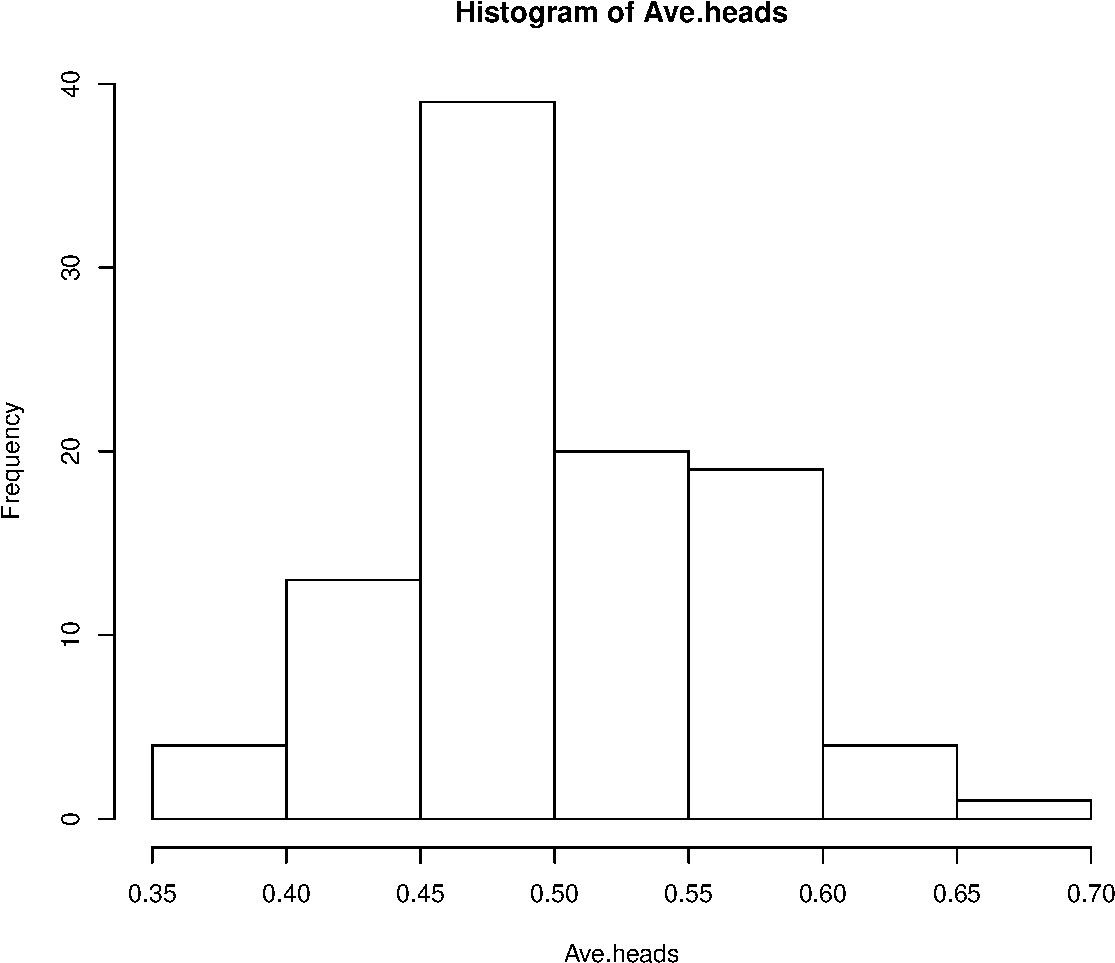
\includegraphics{class2-jan11_files/figure-beamer/unnamed-chunk-10-1.pdf}

\end{frame}

\begin{frame}{Central Limit Theorem}

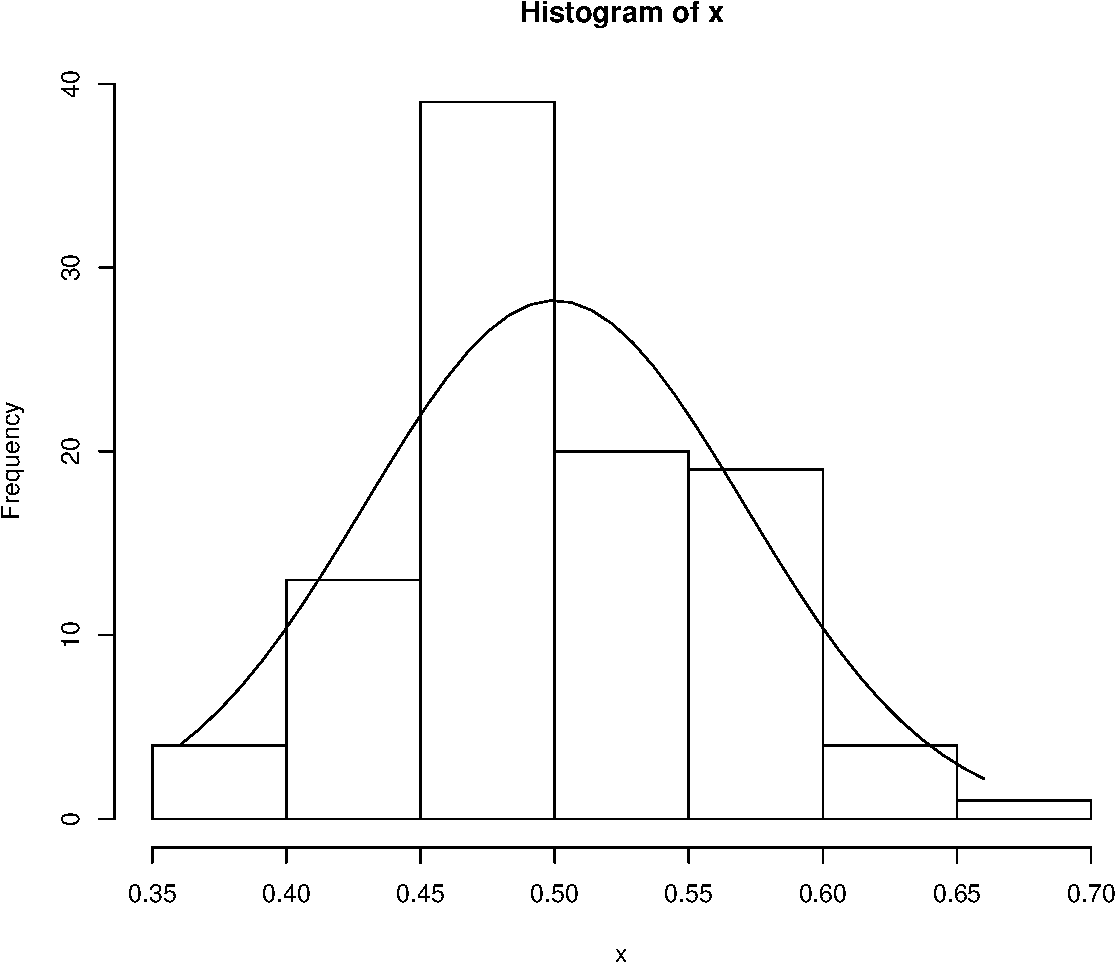
\includegraphics{class2-jan11_files/figure-beamer/unnamed-chunk-11-1.pdf}

\end{frame}

\begin{frame}{Chi-Square Distribution}

Let \(X_1, X_2, ..., X_n\) be independent and identically distributed
random variables that have a \(N(0,1)\) distribution. The distribution
of

\[ \sum_{i=1}^{n}X_i^2,\]

has a chi-square distribution on \(n\) degrees of freedom or
\(\chi^2_{n}\).

The mean of a \(\chi^2_{n}\) is \(n\) with variance \(2n\).

\end{frame}

\begin{frame}{Chi-Square Distribution}

Let \(X_1,X_2,...,X_n\) be independent with a \(N(\mu, \sigma^2)\)
distribution. What is the distribution of the sample variance
\(S^2=\sum_{i=1}^{n}(X_i-{\bar X})^2/(n-1)\)?

\end{frame}

\begin{frame}{t Distribution}

If \(X \sim N(0,1)\) and \(W \sim \chi^2_n\) then the distribution of
\(\frac{X}{\sqrt{W/n}}\) has a t distribution on \(n\) degrees of
freedom or \(\frac{X}{\sqrt{W/{n}}} \sim t_n\).

\end{frame}

\begin{frame}{t Distribution}

Let \(X_1, X_2, ...\) is an independent sequence of identically
distributed random variables that have a \(N(0,1)\) distribution. What
is the distribution of

\[ \frac{{\bar X}-\mu }{\frac {S}{\sqrt {n-1}}}\]

where \(S^2=\sum_{i=1}^{n}(X_i-{\bar X})^2/(n-1)\)?

\end{frame}

\begin{frame}{t Distribution}

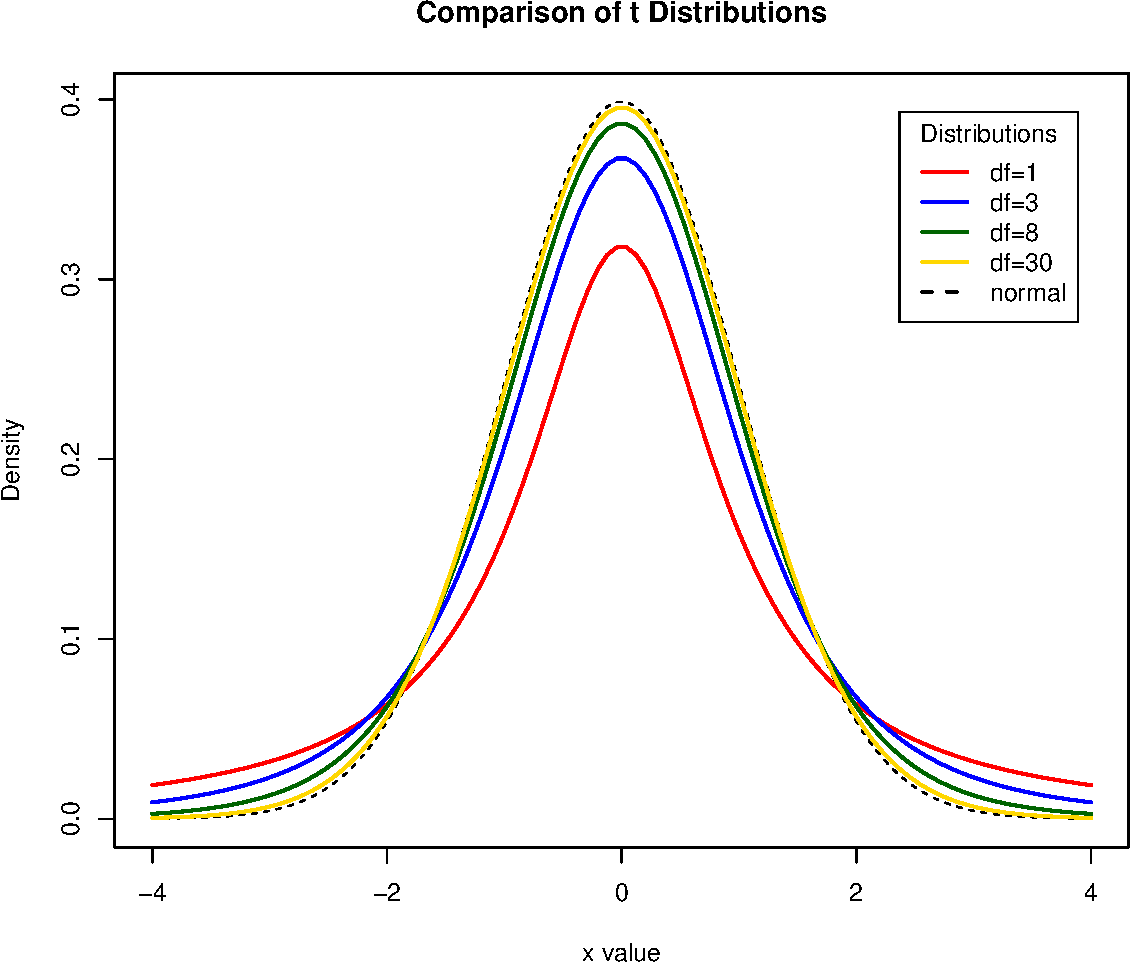
\includegraphics{class2-jan11_files/figure-beamer/unnamed-chunk-12-1.pdf}

\end{frame}

\begin{frame}{F Distribution}

Let \(X \sim \chi^2_m\) and \(Y\sim \chi^2_n\) be independent. The
distribution of

\[ W= \frac{X/m}{Y/n} \sim F_{m,n},\]

where \(F_{m,n}\) denotes the F distribution on \(m,n\) degrees of
freedom. The F distribution is right skewed (see graph below). For
\(n>2, E(W)=n/(n-2)\). It also follows that the square of a \(t_n\)
random variable follows an \(F_{1,n}\).

\end{frame}

\begin{frame}{F Distribution}

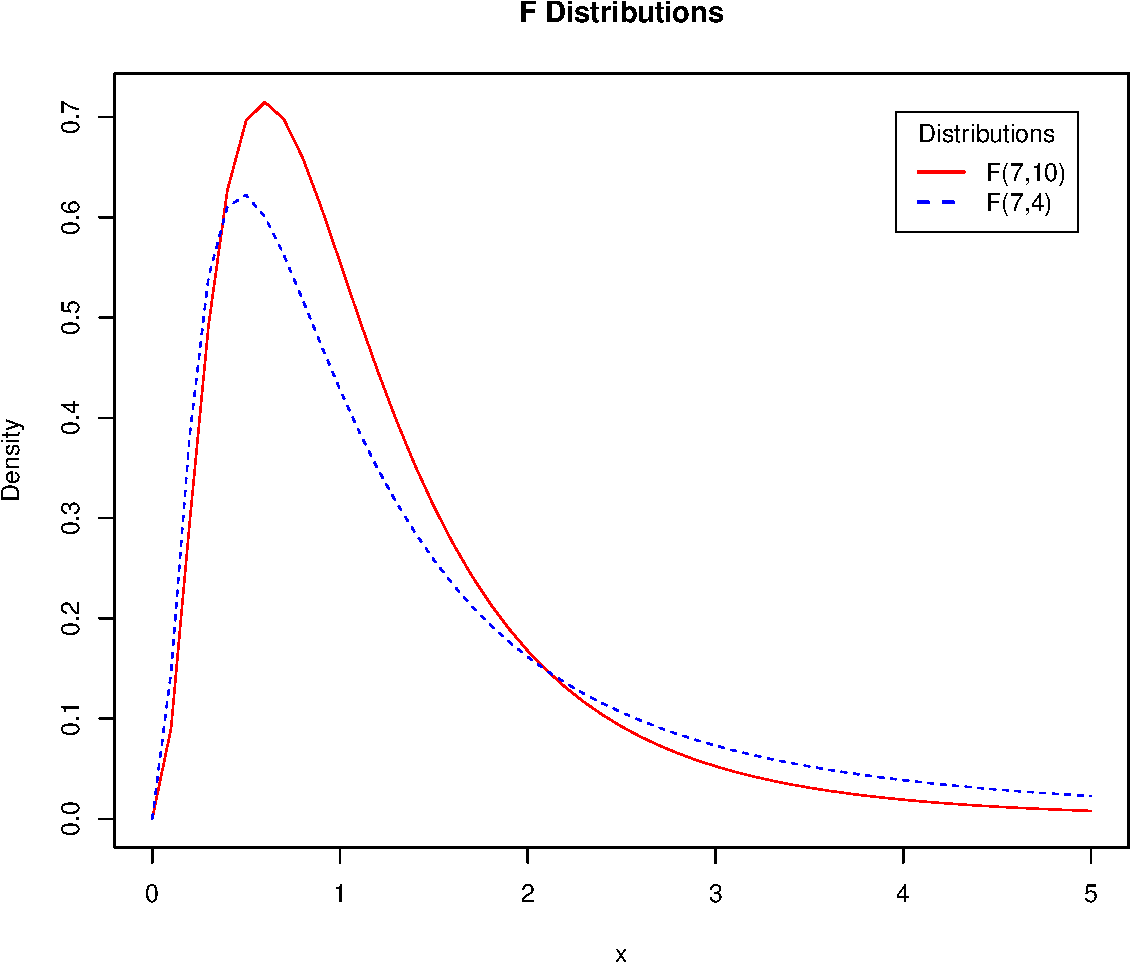
\includegraphics{class2-jan11_files/figure-beamer/unnamed-chunk-13-1.pdf}

\end{frame}

\begin{frame}[fragile]{Linear Regression}

Lea (1965) discussed the relationship between mean annual temperature
and mortality index for a type of breast cancer in women taken from
regions in Europe (example from Wu and Hammada).

The data is shown below.

\begin{Shaded}
\begin{Highlighting}[]
\CommentTok{#Breast Cancer data}
\NormalTok{M <-}\StringTok{ }\KeywordTok{c}\NormalTok{(}\FloatTok{102.5}\NormalTok{, }\FloatTok{104.5}\NormalTok{, }\FloatTok{100.4}\NormalTok{, }\FloatTok{95.9}\NormalTok{, }\FloatTok{87.0}\NormalTok{, }\FloatTok{95.0}\NormalTok{, }\FloatTok{88.6}\NormalTok{, }\FloatTok{89.2}\NormalTok{, }
       \FloatTok{78.9}\NormalTok{, }\FloatTok{84.6}\NormalTok{, }\FloatTok{81.7}\NormalTok{, }\FloatTok{72.2}\NormalTok{, }\FloatTok{65.1}\NormalTok{, }\FloatTok{68.1}\NormalTok{, }\FloatTok{67.3}\NormalTok{, }\FloatTok{52.5}\NormalTok{)}
\NormalTok{T <-}\StringTok{ }\KeywordTok{c}\NormalTok{(}\FloatTok{51.3}\NormalTok{, }\FloatTok{49.9}\NormalTok{, }\FloatTok{50.0}\NormalTok{,}\FloatTok{49.2}\NormalTok{, }\FloatTok{48.5}\NormalTok{, }\FloatTok{47.8}\NormalTok{, }\FloatTok{47.3}\NormalTok{, }\FloatTok{45.1}\NormalTok{, }
       \FloatTok{46.3}\NormalTok{, }\FloatTok{42.1}\NormalTok{, }\FloatTok{44.2}\NormalTok{, }\FloatTok{43.5}\NormalTok{, }\FloatTok{42.3}\NormalTok{, }\FloatTok{40.2}\NormalTok{, }\FloatTok{31.8}\NormalTok{, }\FloatTok{34.0}\NormalTok{)}
\end{Highlighting}
\end{Shaded}

\end{frame}

\begin{frame}{Linear Regression}

A linear regression model of mortality versus temperature is obtained by
estimating the intercept and slope in the equation:

\[ y_i = \beta_0 + \beta_1 x_i + \epsilon_i, i=1,...,n\]

where \(\epsilon_i \sim N(0,\sigma^2)\). The values of
\(\beta_0, \beta_1\) that minimize the sum of squares

\[ \sum_{i=1}^{n} (y_i-(\beta_0+\beta_1 x_i))^2, \]

are called the least squares estimators. They are given by:

\begin{itemize}
\tightlist
\item
  \(\hat{\beta_0}={\bar y}-{\hat{\beta_1}}{\bar{x}}\)
\item
  \({\hat{\beta_1}}=r\frac{S_y}{S_x}\)
\end{itemize}

\(r\) is the correlation between \(y\) and \(x\), and \(S_x, S_y\) are
the sample standard deviations of \(x\) and \(y\) respectively.

\end{frame}

\begin{frame}[fragile]{Linear Regression}

\begin{Shaded}
\begin{Highlighting}[]
\KeywordTok{plot}\NormalTok{(T,M,}\DataTypeTok{xlab=}\StringTok{"temperature"}\NormalTok{,}\DataTypeTok{ylab=}\StringTok{"mortality index"}\NormalTok{)}
\end{Highlighting}
\end{Shaded}

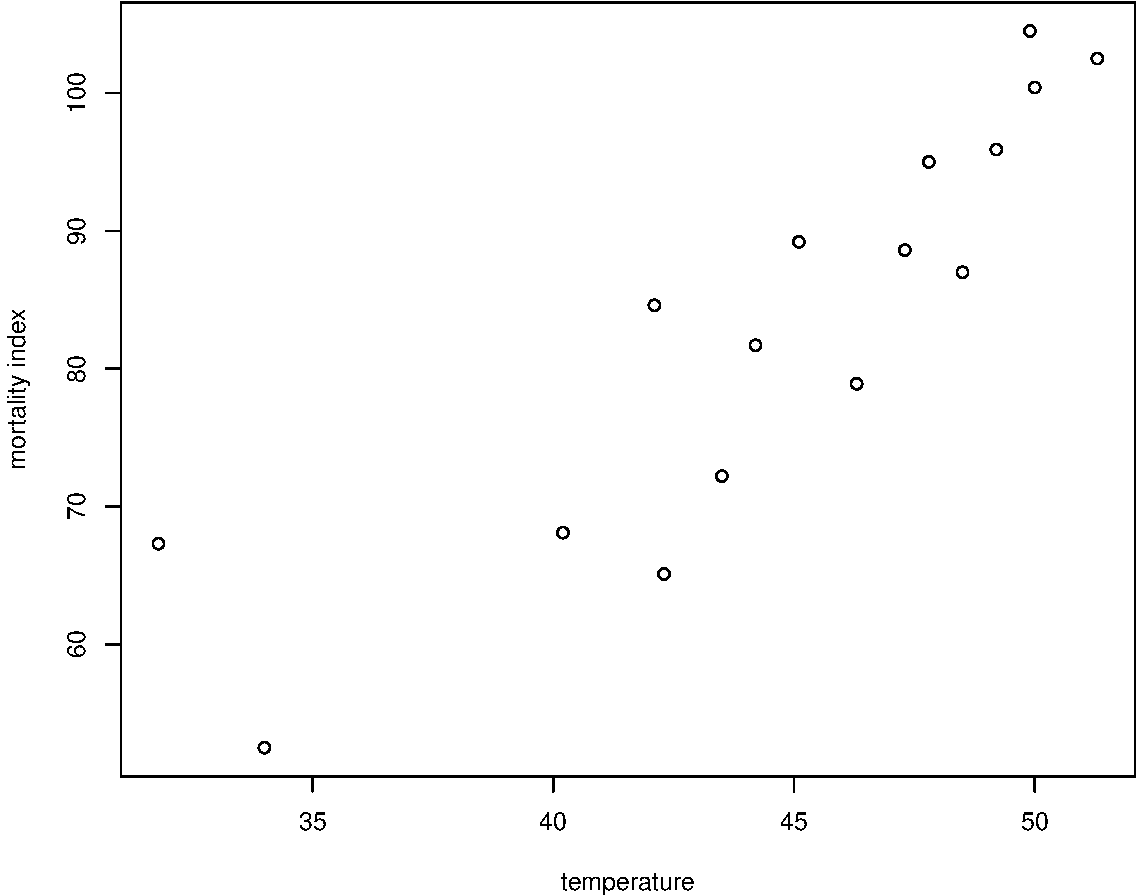
\includegraphics{class2-jan11_files/figure-beamer/unnamed-chunk-15-1.pdf}

\end{frame}

\begin{frame}[fragile]{Linear Regression}

\begin{Shaded}
\begin{Highlighting}[]
\NormalTok{reg1 <-}\StringTok{ }\KeywordTok{lm}\NormalTok{(M~T)}
\KeywordTok{summary}\NormalTok{(reg1) }\CommentTok{# Parameter estimates and ANOVA table}
\end{Highlighting}
\end{Shaded}

\begin{verbatim}
## 
## Call:
## lm(formula = M ~ T)
## 
## Residuals:
##      Min       1Q   Median       3Q      Max 
## -12.8358  -5.6319   0.4904   4.3981  14.1200 
## 
## Coefficients:
##             Estimate Std. Error t value Pr(>|t|)    
## (Intercept) -21.7947    15.6719  -1.391    0.186    
## T             2.3577     0.3489   6.758  9.2e-06 ***
## ---
## Signif. codes:  0 '***' 0.001 '**' 0.01 '*' 0.05 '.' 0.1 ' ' 1
## 
## Residual standard error: 7.545 on 14 degrees of freedom
## Multiple R-squared:  0.7654, Adjusted R-squared:  0.7486 
## F-statistic: 45.67 on 1 and 14 DF,  p-value: 9.202e-06
\end{verbatim}

\end{frame}

\begin{frame}[fragile]{Linear Regression}

\begin{Shaded}
\begin{Highlighting}[]
\KeywordTok{plot}\NormalTok{(T,M,}\DataTypeTok{xlab=}\StringTok{"temperature"}\NormalTok{,}\DataTypeTok{ylab=}\StringTok{"mortality index"}\NormalTok{)}
\KeywordTok{abline}\NormalTok{(reg1) }\CommentTok{# Add regression line to the plot}
\end{Highlighting}
\end{Shaded}

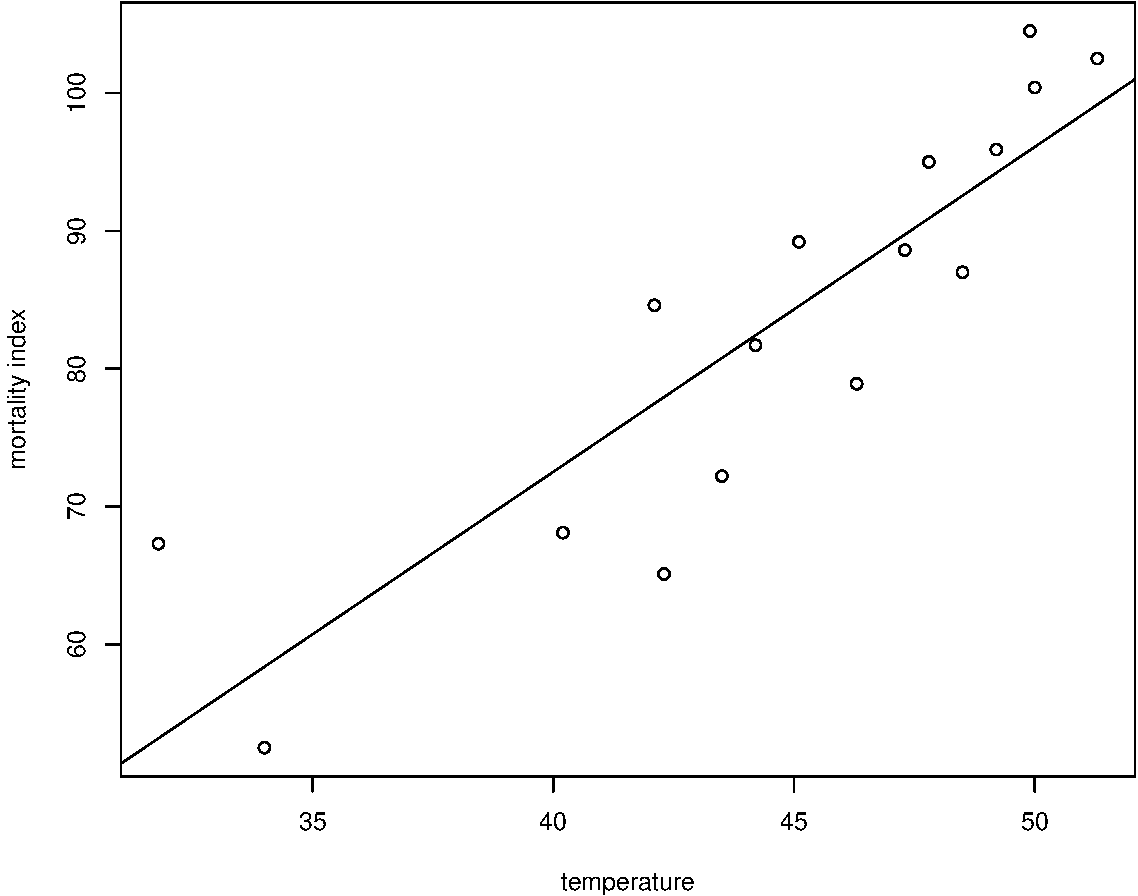
\includegraphics{class2-jan11_files/figure-beamer/unnamed-chunk-17-1.pdf}

\end{frame}

\begin{frame}[fragile]{Linear Regression}

\begin{Shaded}
\begin{Highlighting}[]
\CommentTok{#plot residuals vs. fitted}
\KeywordTok{plot}\NormalTok{(reg1$fitted,reg1$residuals);}
\KeywordTok{abline}\NormalTok{(}\DataTypeTok{h=}\DecValTok{0}\NormalTok{) }\CommentTok{# add horizontal line at 0}
\end{Highlighting}
\end{Shaded}

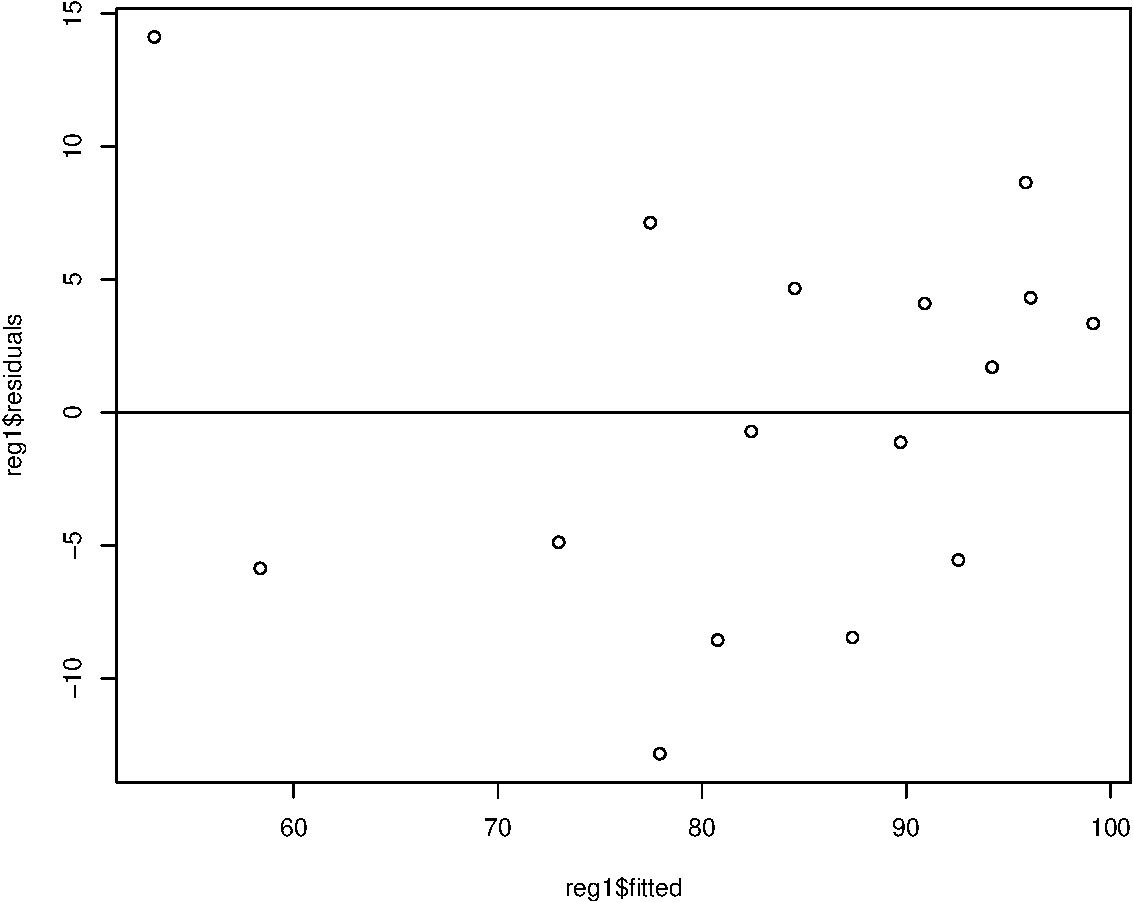
\includegraphics{class2-jan11_files/figure-beamer/unnamed-chunk-18-1.pdf}

\end{frame}

\begin{frame}[fragile]{Linear Regression}

\begin{Shaded}
\begin{Highlighting}[]
\CommentTok{#check normality of residuals}
\KeywordTok{qqnorm}\NormalTok{(reg1$residuals); }\KeywordTok{qqline}\NormalTok{(reg1$residuals)}
\end{Highlighting}
\end{Shaded}

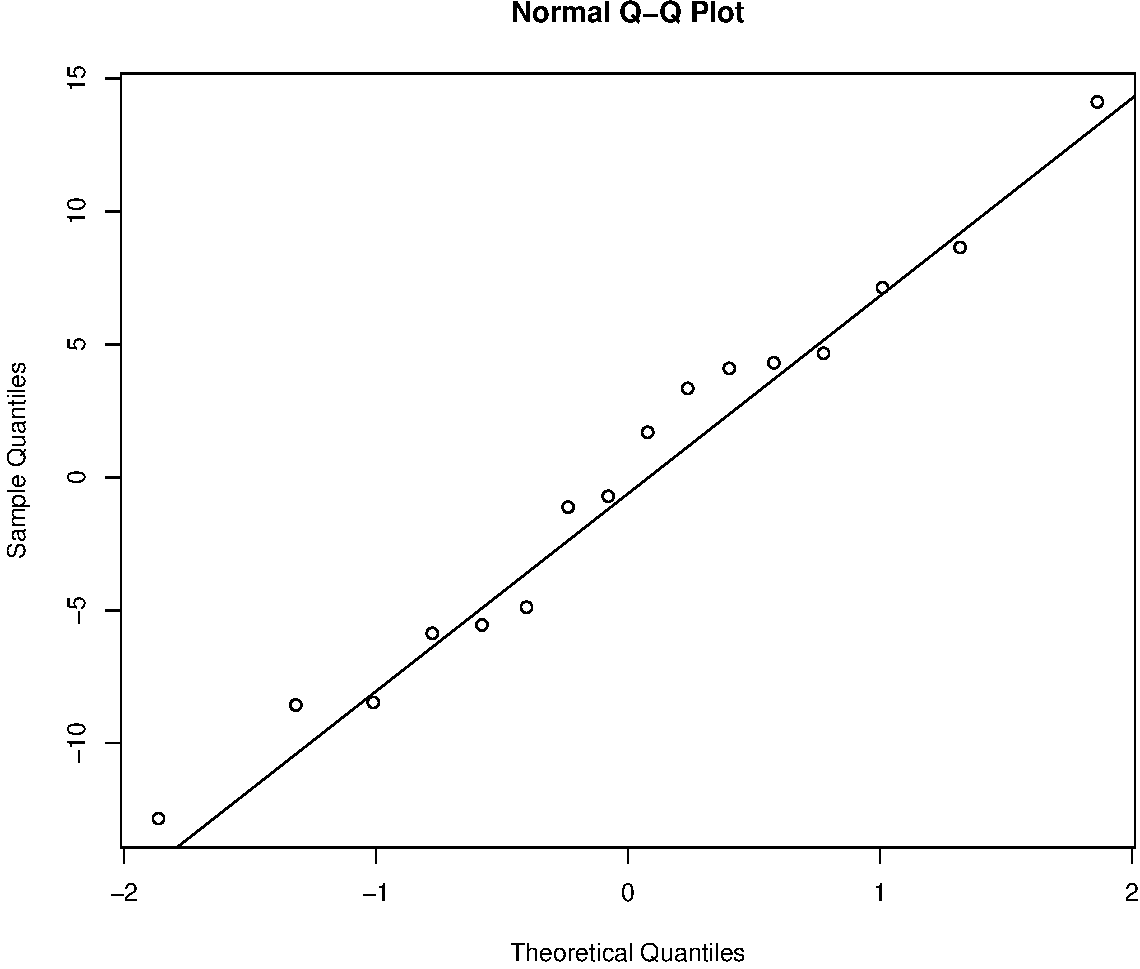
\includegraphics{class2-jan11_files/figure-beamer/unnamed-chunk-19-1.pdf}

\end{frame}

\begin{frame}{Linear Regression}

If there is more than one independent variable then the above model is
called a multiple linear regression model.

\[ y_i=\beta_0+\beta_1 x_{i1} + \beta_2 x_{i2} + \cdots +  \beta_k x_{ik} + \epsilon_{i}, \thinspace i=1,...,n, \]

where \(\epsilon_{i} \sim N(0,\sigma^2)\).

This can also be expressed in matrix notation as

\[ y=X\beta+\epsilon\]

The least squares estimator is

\[{\hat \beta}=\left(X^{T} X\right)^{-1}X^{T}y.\]

The covariance matrix of \({\hat \beta}\) is
\(\left(X^{T} X\right)^{-1}{\sigma}^2\). An estimator of \(\sigma^2\) is

\[{\hat \sigma^2}=\frac{1}{n-k}\sum_{i=1}^{n}(y_i-{\hat y_i})^2,\]

where
\({\hat y_i}={\hat \beta_0}+{\hat \beta_1} x_{i1} + \cdots + {\hat \beta_k} x_{ik}\)
is the predicted value of \(y_i\).

\end{frame}

\begin{frame}{Weighing Problem}

Harold Hotelling in 1949 wrote a paper on how to obtain more accurate
weighings through experimental design.

\textbf{Method 1}

Weigh each apple separately.

\textbf{Method 2}

Obtain two weighings by

\begin{enumerate}
\def\labelenumi{\arabic{enumi}.}
\tightlist
\item
  Weighing two apples in one pan.
\item
  Weighing one apple in one pan and the other apple in the other pan
\end{enumerate}

\end{frame}

\begin{frame}{Weighing Problem}

Let \(w_1, w_2\) be the weights of apples one and two. Each weighing has
standard error \(\sigma\). So the precision of the estimates from method
1 is \(\sigma\).

If the objects are weighed together in one pan, resulting in measurement
\(m_1\), then in opposite pans, resulting in measurement \(m_2\), we
have two equations for the unknown weights \(w_1,w_2\):

\[w_1+w_2 =  m_1\] \[w_1-w_2 =  m_2\]

\end{frame}

\begin{frame}{Weighing Problem}

This can also be viewed as a linear regression problem
\(y=X{\beta}+\epsilon\):

\[y=(m_1,m_2)^{\prime},\thinspace X=
 \begin{pmatrix}
  1 & 1 \\
  1 & -1 \\
 \end{pmatrix}, \thinspace {\beta}=(w_1,w_2)^{\prime}.\]

\end{frame}

\begin{frame}[fragile]{Weighing Problem}

The least-squares estimates can be found using R.

\begin{Shaded}
\begin{Highlighting}[]
\CommentTok{#step-by-step matrix mutiplication example for weighing problem}

\NormalTok{X <-}\StringTok{ }\KeywordTok{matrix}\NormalTok{(}\KeywordTok{c}\NormalTok{(}\DecValTok{1}\NormalTok{,}\DecValTok{1}\NormalTok{,}\DecValTok{1}\NormalTok{,-}\DecValTok{1}\NormalTok{),}\DataTypeTok{nrow=}\DecValTok{2}\NormalTok{,}\DataTypeTok{ncol=}\DecValTok{2}\NormalTok{) }\CommentTok{#define X matrix}
\NormalTok{Y <-}\StringTok{ }\KeywordTok{t}\NormalTok{(X)%*%X }\CommentTok{# multiply X^T by X (X^T*X) NB: t(X) is transpose of X}
\NormalTok{W <-}\StringTok{ }\KeywordTok{solve}\NormalTok{(Y) }\CommentTok{# calculate the inverse}
\NormalTok{W %*%}\StringTok{ }\KeywordTok{t}\NormalTok{(X) }\CommentTok{# calculate (X^T*X)^(-1)*X^T}
\end{Highlighting}
\end{Shaded}

\begin{verbatim}
##      [,1] [,2]
## [1,]  0.5  0.5
## [2,]  0.5 -0.5
\end{verbatim}

\begin{Shaded}
\begin{Highlighting}[]
\NormalTok{W }\CommentTok{# print (X^T*X)^(-1) for SE }
\end{Highlighting}
\end{Shaded}

\begin{verbatim}
##      [,1] [,2]
## [1,]  0.5  0.0
## [2,]  0.0  0.5
\end{verbatim}

\end{frame}

\end{document}
